\section{Data Flow Experiments}
\label{sec:dataflow_experiments}

Data flow analysis is at the heart of modern compiler technology. We pose a
suite of data flow analyses as supervised learning tasks to benchmark the
representational power of machine learning approaches. We selected a diverse set
of tasks that capture a mixture of both forward and backward analyses, and
control-, data-, and procedure-sensitive analyses. \emph{Full details of the
analyses are provided in Appendix A.} These particular data flow analyses can
already be perfectly solved by non-ML techniques. Here, we use them to benchmark
the capabilities of machine learning techniques.

\subsection{The \textsc{DeepDataFlow} Dataset}
\label{subsec:dataset}

We assembled a 256M-line corpus of LLVM-IR files from a variety of sources and
produced labeled datasets using five traditional data flow analyses: control
reachability, dominators, data dependencies, liveness, and
subexpressions~\cite{chris_cummins_2020_4247595}. Each of the 15.4M analysis
examples consists of an input graph in which a single vertex is annotated as the
root node for analysis, and an output graph in which each vertex is annotated
with a binary label corresponding to its value once the data flow analysis has
completed (Fig.~\ref{fig:dataflow_examples}). A 3:1:1 ratio is used to divide
the examples for the five problems into training, validation, and test
instances. When formulated as supervised learning tasks, data flow analyses
exhibit a strong class imbalance. A trivial baseline is to always predict
\emph{true}, which achieves an F$_1$ of 0.073.  \emph{For further details see
Appendix~B.}

\begin{figure*}
  \centering
  \begin{subfigure}{.19\linewidth}
    \includegraphics[width=\linewidth]{images/dataflow/A_reachability}%
    \caption{\textsc{Reachability}}
    \label{subfig:dataflow_reachability}
  \end{subfigure}
  \hfill
  \begin{subfigure}{.19\linewidth}
    \includegraphics[width=\linewidth]{images/dataflow/B_dominance}%
    \caption{\textsc{Dominance}}
    \label{subfig:dataflow_dominance}
  \end{subfigure}
  \hfill
  \begin{subfigure}{.19\linewidth}
    \includegraphics[width=\linewidth]{images/dataflow/C_datadep}%
    \caption{\textsc{DataDep}}
    \label{subfig:dataflow_datadep}
  \end{subfigure}
  \hfill
  \begin{subfigure}{.19\linewidth}
    \includegraphics[width=\linewidth]{images/dataflow/D_liveness}%
    \caption{\textsc{Liveness}}
    \label{subfig:dataflow_liveness}
  \end{subfigure}
  \hfill
  \begin{subfigure}{.21\linewidth}
    \includegraphics[width=.97\linewidth]{images/dataflow/E_subexpressions}%
    \caption{\textsc{Subexpressions}}
    \label{subfig:dataflow_subexpressions}
  \end{subfigure}
  \caption{%
    Example input-output graphs for each of the five \textsc{DeepDataFlow}
    tasks. A single vertex is randomly selected from the input graph as the
    starting point for computing analysis results, indicated using the
    \emph{vertex selector} (blue node). Each vertex in the output graph is
    annotated with a binary value after the analysis has completed. As a
    supervised classification task, the goal is to predict the output vertex
    labels given an input graph. These small graphs are for illustrative
    purposes, the average \textsc{DeepDataFlow} graph contains 581 vertices and
    1,051 edges.%
   }
  \label{fig:dataflow_examples}%
\end{figure*}

\subsection{Models}%
\label{subsubsec:dataflow_models}

We evaluate the effectiveness of our approach against two contrasting
state-of-the-art approaches for learning over programs: one sequential model and
one other graph model.

\paragraph{(I) Sequential Model}%
\emph{inst2vec}~\citep{Ben-nun2018} sequentially processes the IR statements of
a program to perform whole-program classification. An IR is tokenized and then
mapped into a sequence of pre-trained 200 dimensional embedding vectors which
are processed by an LSTM. The final state of the LSTM is fed through a two-layer
fully connected neural network to produce a classification of the full sequence.
We extend this approach by concatenating to the input sequence a one-hot
\emph{token-selector} to indicate the starting point for analysis. Then, we feed
the LSTM state through a fully connected layer after every token, producing a
prediction for each instruction of the IR. We use the same model parameters as
in the original work.

\paragraph{(II) Graph Models}%
We use the model design outlined in
Section~\ref{sec:graph-based-machine-learning} with two input representations:
CDFG~\citep{Brauckmann2020}, and \programl. For both approaches we use 32
dimensional embeddings initialized randomly, as in~\citet{Brauckmann2020}. Input
\emph{vertex-selectors}, encoded as binary one-hot vectors, are used to mark the
starting point for analyses and are concatenated to the initial embeddings. For
CDFG, we use the vocabulary described in~\citet{Brauckmann2020}. For \programl,
we derive the vocabulary from the training set.

Message Passing Neural Networks typically use a small number of propagation
steps out of practical consideration for time and space
efficiency~\citep{Gilmer2017,Brauckmann2020}. In contrast, data flow analyses
iterate until a fixed point is reached. In this work we iterate for a fixed
number $T$ of message passing steps and exclude from the training and validation
sets graphs for which a traditional implementation of the analysis task requires
greater than $T$ iterations to solve. We set $T = 30$ for training in all
experiments and trained a model per task. Once trained, we evaluate model
inference using different $T$ values to accommodate programs which required a
greater number of steps to compute the ground truth. \emph{See Appendix~C.2. for
training details.}

\begin{figure*}[!t]
\vspace{1em}
\begin{minipage}[T]{\textwidth}
    \begin{minipage}[b]{.27\linewidth}
        \centering%
\scriptsize
\begin{tabular}{r R{1.2cm} R{1.4cm}}
  & Vocabulary Size & Vocabulary Test Coverage \\
  \toprule
  inst2vec & 8,565 & 34.0\%\\
  CDFG & 75 & 47.5\% \\
  \programl & 2,230 & \textbf{98.3\%} \\
  &&\\
\end{tabular}

        \label{tab:vocabularies}
        \captionof{table}{Vocabularies for LLVM-IR.}%
    \end{minipage}
    \hfill
    \begin{minipage}[b]{.61\linewidth}
        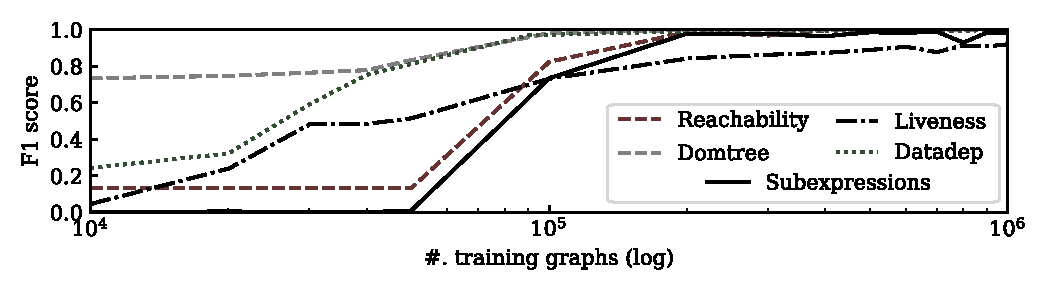
\includegraphics[width=\linewidth]{images/programl-f1.pdf}
        \vspace{-2em}
        \captionof{figure}{%
          F$_1$ score on a 10k-graph validation set as a function of the
          number of training graphs.%
        }
        \label{fig:dataflow_convergence}
    \end{minipage}
\end{minipage}
\end{figure*}

\begin{table*}[t]
  \centering%
  \vspace{.5em}
\footnotesize
\begin{tabular}{l L{4cm} r c c | c : c c}
  Analysis & Example Optimization &  & inst2vec & CDFG & \multicolumn{3}{c}{\programl} \\
   & & & DDF-30  & DDF-30 & DDF-30 & DDF-60 & \ddfinf{}\\
  \toprule
Reachability &
\multirow{2}{2.1cm}{Dead Code Elimination}
        & Precision  &  0.105  & \textbf{1.000}  &  0.998 & 0.997 & 0.996  \\
       & & Recall  &  0.007  & 0.996  &  \textbf{0.998}  & 0.998 & 0.917 \\
  \vspace{.3em}
        & & F$_1$  &  0.012  & \textbf{0.998}  &  \textbf{0.998} & 0.997 & 0.943 \\
Dominance &
Global Code Motion
        & Precision  &  0.053  &  0.999  &  \textbf{1.000} & 0.983 & 0.066 \\
       & & Recall  &  0.002  &  \textbf{1.000}  &  \textbf{1.000} & 1.000 & 0.950 \\
  \vspace{.3em}
        & & F$_1$  &  0.004  &  0.999  &  \textbf{1.000} & 0.991 & 0.123 \\
DataDep &
Instruction Scheduling
        & Precision  &  ---    &  ---    &  \textbf{0.998} & 0.992 & 0.987 \\
       & & Recall  &  ---    &  ---    &  \textbf{0.997} & 0.996 & 0.949 \\
  \vspace{.3em}
        & & F$_1$  &  ---    &  ---    &  \textbf{0.997} & 0.993 & 0.965 \\
Liveness &
Register Allocation
        & Precision  &  ---    &  ---    &  \textbf{0.962} & 0.931 & 0.476 \\
       & & Recall  &  ---    &  ---    &  \textbf{0.916} & 0.955 & 0.925 \\
  \vspace{.3em}
        & & F$_1$  &  ---    &  ---    &  \textbf{0.937} & 0.939 & 0.625 \\
Subexpressions &
\multirow{3}{3cm}{Global Common Subexpression Elimination}
        & Precision  &  0.000  &  0.139   &  \textbf{0.997}  & 0.954 & 0.938 \\
       & & Recall  &  0.000  &  0.005  &  \textbf{0.996}  & 0.999 & 0.992 \\
       & & F$_1$  &  0.000  &  0.009   &  \textbf{0.996} & 0.967 & 0.959 \\
\end{tabular}
\vspace{-1em}
%
  \vspace{.4em}
  \caption{%
    Data flow analysis results. For the restricted subset DDF-30 \programl
    obtains strong results. Results on the full dataset (DDF) highlight the
    scalability challenges of MPNNs.%
  }%
  \label{table:data_flow_results} %
\end{table*}

\subsection{Evaluation}

First, we evaluate the effectiveness of each vocabulary at representing unseen
programs. Then we evaluate model performance on increasingly large subsets of
the \textsc{DeepDataFlow} (DDF) test sets.

\paragraph{Vocabulary Coverage} Each of the three approaches uses a vocabulary
to produce embeddings that describe the instructions and operands of a program.
inst2vec uses a vocabulary of 8,565 LLVM-IR statements (where a statement is an
instruction and its operands) with identifiers and literals stripped.  CDFG uses
the 75 LLVM instruction opcodes. For \programl we derive a vocabulary on a set
of training graphs that represents instructions and data types separately. Table
1 compares the coverage of these vocabularies as a percentage of the vertices in
the test graphs that can be described using that vocabulary.  \programl provides
$2.1\times$ the coverage on unseen programs as state-of-the-art approaches, the
best of which can represent fewer than half of the graph vertices of unseen
programs.

\paragraph{DDF-30: Testing on Limited Problem Size} We initially limit our
testing to the subset of each task's test set which can be solved using a
traditional analysis implementation in $\le 30$ steps, denoted DDF-30. This
matches the $T = 30$ message passing iterations used in computing the graph
models' final states to ensure that a learned model, if it has successfully
approximated the mechanism of an analysis, has sufficient message passing
iterations to solve each test input. Table~\ref{table:data_flow_results}
summarizes the performance of inst2vec, CDFG, and \programl.

The relational representation of our approach shows excellent performance across
all of the tasks. CDFG, which also captures control-flow, achieves comparable
performance on the \textsc{Reachability} and \textsc{Dominance} tasks. However,
the lack of operand vertices, positional edges, and data types renders poor
performance on the \textsc{Subexpressions} task. Neither CDFG nor inst2vec
representations enable per-variable classification, so are incapable of the
\textsc{DataDep} and \textsc{Liveness} tasks. To simplify comparison, we exclude
these two tasks from inst2vec and CDFG aggregate scores. In spite of this,
\programl correctly labels  $4.50\times$ and $1.12\times$ more vertices than the
state-of-the-art approaches. The weakest \programl performance is on the
\textsc{Liveness} task. When model performance is considered as a function of
the number of training graphs, shown in Figure~\ref{fig:dataflow_convergence},
we see that the performance of \programl quickly converges towards near-perfect
$F_1$ scores on a holdout validation set for all tasks except \textsc{Liveness},
where the model is still improving at the end of training. This suggests
estimating the \emph{transfer} (message) and \emph{meet} (update) operators of
this backwards analysis poses a greater challenge for the network, and may
benefit from further training.

\paragraph{DDF-60: Generalizing to Larger Problems} The DDF-30 set excludes
28.7\% of \textsc{DeepDataFlow} graphs which require more than 30 steps to
compute ground truth labels. To test whether these learned models can generalize
to solve larger problems, we used the models we trained at $T=30$ but double the
number of inference message passing steps to $T=60$ and repeated the tests on
all graphs which require $\le$ 60 analysis steps (excluding 19.6\%). The results
of this experiment, denoted DDF-60, are shown in
Table~\ref{table:data_flow_results}. We observe that performance is consistent
on this larger problem set, demonstrating that \programl models can generalize
to problems larger than those they were trained on. The results indicate that an
approximate fixed-point algorithm is learned by the model, a critical feature
for enabling practical machine learning over programs.


\paragraph{\ddfinf{}: Scalability Challenges} Finally, we test the analysis
models that were trained for $T=30$ message passing iterations on all
\textsc{DeepDataFlow} graphs, shown in Table~\ref{table:data_flow_results} as
\ddfinf{}. We use $T=200$ inference message passing iterations to test the
limits of stability and generalization of current graph neural networks,
irrespective of the number of steps required to compute ground truth labels,
whereas 9.6\% of \ddfinf{} graphs require more than 200 steps to compute.
Therefore, this experiment highlights two of the challenges in the formulation
of data flow analysis in an MPNN framework: first, that using a fixed number of
message passing iterations across each and every edge leads to unnecessary work
for problems that can be solved in fewer iterations or by propagating only along
a dynamic subset of the edges at each timestep (the maximum number of steps
required by a graph in \ddfinf{} is 28,727). Secondly, models that compute
correct results for a graph when processed for an appropriate number of steps
may prove unstable when processed for an excessively large number of steps. In
Table~\ref{table:data_flow_results} we see substantial degradations of model
performance in line with these two challenges. \textsc{Dominance} and
\textsc{Liveness} show reductions in precision as the models over-approximate
and have a large number of false positives. \textsc{Reachability} and
\textsc{DataDep}, in contrast, show drops in recall as the fixed $T=200$
iterations is insufficient to propagate the signal to the edges of large
problems.

MPNNs do not scale in the way that we should like for large programs. A part of
this, we believe, is that using a generic MPNN system is wasteful. Ordinary data
flow engines process nodes in a particular order (usually reverse post order)
and are naturally able to identify that a fixed point has been reached. We
believe that \emph{dynamically-sparse} message passing strategies and an
adaptive number of iterations could address these scalability challenges, which
we will pursue in future work.
